\documentclass{beamer}

% Theme and packages
\usetheme{CambridgeUS}
\usecolortheme{default}
\usepackage[utf8]{inputenc}
\usepackage{graphicx}
\usepackage{booktabs}
\usepackage{tikz}
\usepackage{fontawesome5}
\usepackage{hyperref}
\usepackage{multicol}
\usepackage{xcolor}

% Custom colours
\definecolor{aiblue}{RGB}{79, 195, 247}
\definecolor{darkblue}{RGB}{1, 87, 155}
\definecolor{successgreen}{RGB}{76, 175, 80}
\definecolor{warningorange}{RGB}{255, 152, 0}

% Custom commands for better formatting
\newcommand{\highlight}[1]{\textcolor{aiblue}{\textbf{#1}}}

\title{AI-Powered Knowledge Work}
\subtitle{Master the New Universal Workspace}
\author{Dr. John O'Hare}
\institute{DREAMLAB | HP AI Lighthouse Partner}
\date{2025}

% Command to set background
\usebackgroundtemplate{%
    \includegraphics[width=\paperwidth,height=\paperheight]{placeholder.png}%
}

\setbeamertemplate{background canvas}{
    \ifnum\thepage>0
        \begin{tikzpicture}[remember picture, overlay]
            \node[at=(current page.center), opacity=0.3] {
                \includegraphics[width=\paperwidth,height=\paperheight]{slide-\thepage-backdrop.png}
            };
        \end{tikzpicture}
    \fi
}

\begin{document}

% Title slide
\begin{frame}[plain]
% Image prompt: Futuristic workspace with holographic AI interfaces, VS Code prominently displayed on multiple screens, diverse professionals collaborating, modern office setting with glass walls, blue and white colour scheme, photorealistic style
\titlepage
\end{frame}

% Executive Summary - The Revolution
\begin{frame}{The AI Revolution in Knowledge Work}
% Image prompt: Split screen showing traditional office worker drowning in paperwork on left vs empowered professional with AI assistants visualised as glowing orbs on right, dramatic lighting, business setting
\begin{block}{The Paradigm Shift}
The boundary between "technical" and "non-technical" work has \highlight{dissolved}.
\end{block}
\vspace{0.5em}
\begin{columns}[T]
\begin{column}{0.48\textwidth}
\textbf{Before:}
\begin{itemize}
\item Copy-paste from ChatGPT
\item Limited by web interfaces
\item No version control
\item Manual repetitive tasks
\end{itemize}
\end{column}
\begin{column}{0.48\textwidth}
\textbf{After This Workshop:}
\begin{itemize}
\item Direct AI API access
\item VS Code as AI command centre
\item Professional automation
\item 10x productivity gains
\end{itemize}
\end{column}
\end{columns}
\end{frame}

% The Problem/Opportunity
\begin{frame}{The Professional AI Divide}
% Image prompt: Graph showing exponential growth curve with two groups of people - small group soaring upward with AI tools, larger group stuck at bottom with basic tools, clean infographic style
\begin{center}
\Large{Two Classes of AI Users Are Emerging}
\end{center}
\vspace{1em}
\begin{itemize}
\item \textbf{The 95\%}: Limited to consumer tools, copy-paste workflows
\item \textbf{The 5\%}: Direct API access, automation, 10x productivity
\end{itemize}
\vspace{1em}
\begin{alertblock}{The Gap Is Widening Daily}
While most struggle with ChatGPT limits, a small group writes books in days, creates comprehensive documentation in hours, and builds autonomous knowledge systems.
\end{alertblock}
\end{frame}

% Who Is This For - Enhanced
\begin{frame}{Transform Your Professional Practice}
% Image prompt: Diverse group of professionals (academic, business executive, consultant, researcher, creative) each with thought bubbles showing their AI-enhanced work outputs, modern illustration style
\begin{columns}[T]
\begin{column}{0.45\textwidth}
\textbf{Perfect For:}
\begin{itemize}
\item Academics \& Researchers
\item Business Leaders
\item Consultants
\item Government \& NGO
\item Creative Professionals
\item Entrepreneurs
\end{itemize}
\end{column}
\begin{column}{0.45\textwidth}
\textbf{If You:}
\begin{itemize}
\item Work with documents daily
\item Feel limited by ChatGPT
\item Need privacy for sensitive data
\item Want to automate repetitive work
\item Are curious about AI's potential
\end{itemize}
\end{column}
\end{columns}
\vspace{0.5em}
\begin{center}
\small{\textit{No coding experience required - if you can use Word, you're ready}}
\end{center}
\end{frame}

% Transformation Journey - Visual
\begin{frame}{Your 5-Day Transformation Journey}
% Image prompt: Ascending staircase or mountain path with 5 glowing waypoints, each showing progression from basic user to AI master, ethereal technological landscape, journey metaphor
\centering
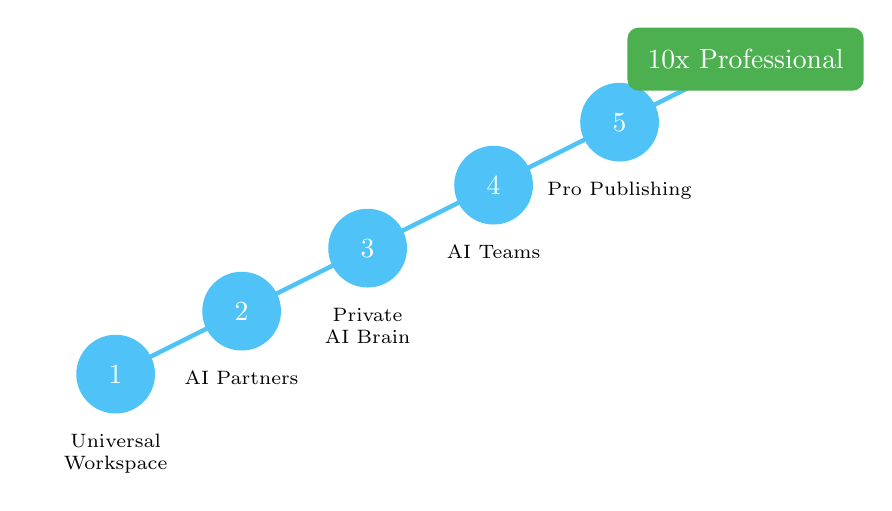
\begin{tikzpicture}[scale=0.8]
% Journey path
\draw[ultra thick, aiblue] (0,0) -- (2,1) -- (4,2) -- (6,3) -- (8,4) -- (10,5);
% Day markers
\foreach \x/\y/\day/\title in {0/0/1/Universal Workspace, 2/1/2/AI Partners, 4/2/3/Private AI Brain, 6/3/4/AI Teams, 8/4/5/Pro Publishing} {
    \node[circle, fill=aiblue, text=white, minimum size=1cm] at (\x,\y) {\day};
    \node[below, text width=2cm, align=center, font=\scriptsize] at (\x,\y-0.8) {\title};
}
% Outcome
\node[rectangle, fill=successgreen, text=white, rounded corners, minimum width=3cm, minimum height=0.8cm] at (10,5) {10x Professional};
\end{tikzpicture}
\vspace{1em}
\textbf{From AI Consumer to AI Commander in 5 Days}
\end{frame}

% Programme Overview - High Level
\begin{frame}{Programme Structure}
% Image prompt: Clean infographic showing 5 interconnected hexagons, each representing a day with icons (workspace, AI brain, team, publishing), modern flat design
\footnotesize
\begin{tabular}{@{}lp{3.5cm}p{5.5cm}p{3cm}@{}}
\toprule
\textbf{Day} & \textbf{Theme} & \textbf{Core Focus} & \textbf{Your Win} \\
\midrule
1 & \highlight{Universal Workspace} & VS Code setup, containers, version control & Professional AI workspace \\
2 & \highlight{AI Creative Partner} & Direct API access, "vibe coding" & Live website via conversation \\
3 & \highlight{Private AI Brain} & Local models, RAG systems & Offline knowledge base \\
4 & \highlight{AI Teams} & Specialised agents, orchestration & Automated workflows \\
5 & \highlight{Pro Publishing} & LaTeX, websites, automation & Complete portfolio \\
\bottomrule
\end{tabular}
\end{frame}

% Day 1 Deep Dive
\begin{frame}{Day 1: Your Universal AI Workspace}
% Image prompt: VS Code interface with multiple panels showing documents, AI chat, version control, and Mermaid diagrams, clean screenshot style with annotations
\begin{columns}[T]
\begin{column}{0.5\textwidth}
\textbf{Morning: Setup \& Foundations}
\begin{itemize}
\item Transform VS Code into AI command centre
\item Install game-changing extensions
\item Container setup for stability
\item Navigate like a pro
\end{itemize}
\end{column}
\begin{column}{0.5\textwidth}
\textbf{Afternoon: Visual Tools}
\begin{itemize}
\item Mermaid diagrams mastery
\item Version control for ANY document
\item Build your first repository
\item Track every change forever
\end{itemize}
\end{column}
\end{columns}
\vspace{0.5em}
\begin{alertblock}{Day 1 Deliverable}
Professional workspace with visual project plan (Gantt chart) for YOUR real project
\end{alertblock}
\end{frame}

% Day 2 Deep Dive
\begin{frame}{Day 2: AI as Your Creative Partner}
% Image prompt: Split screen showing natural language conversation on left transforming into beautiful website/documents on right, magical transformation effect, modern design
\begin{block}{The "Vibe Coding" Revolution}
Describe what you want in plain English → AI builds it perfectly
\end{block}
\vspace{0.5em}
\begin{columns}[T]
\begin{column}{0.5\textwidth}
\textbf{Morning: Direct AI Access}
\begin{itemize}
\item Connect OpenAI, Claude, Gemini
\item Compare model strengths
\item See real API costs (pennies!)
\item Generate business plans, papers
\end{itemize}
\end{column}
\begin{column}{0.5\textwidth}
\textbf{Afternoon: Build by Talking}
\begin{itemize}
\item Create websites via chat
\item Interactive presentations
\item Data visualisations
\item Deploy live in minutes
\end{itemize}
\end{column}
\end{columns}
\vspace{0.5em}
\textcolor{successgreen}{\faCheckCircle} \textbf{Day 2 Win:} Professional website live on the internet
\end{frame}

% Day 3 Deep Dive
\begin{frame}{Day 3: Your Private AI Brain}
% Image prompt: Secure vault with AI brain inside, documents flowing in and knowledge flowing out, privacy shields, local computer setup, tech-noir style
\begin{alertblock}{Complete Privacy + Total Recall}
AI that knows your entire document history and works 100\% offline
\end{alertblock}
\vspace{0.5em}
\begin{columns}[T]
\begin{column}{0.5\textwidth}
\textbf{Morning: Local AI Models}
\begin{itemize}
\item Install AI on YOUR laptop
\item No internet required
\item Perfect for sensitive data
\item Multiple specialist models
\end{itemize}
\end{column}
\begin{column}{0.5\textwidth}
\textbf{Afternoon: RAG System}
\begin{itemize}
\item Feed in all your documents
\item Instant answers with citations
\item "What was decided in March?"
\item Your personal AI librarian
\end{itemize}
\end{column}
\end{columns}
\vspace{0.5em}
\begin{center}
\small{\textit{Perfect for: Confidential business docs, proprietary research, client data}}
\end{center}
\end{frame}

% Day 4 Deep Dive
\begin{frame}{Day 4: AI Teams Working For You}
% Image prompt: Orchestra of AI agents as glowing entities, each specialised (researcher, writer, analyst), working in harmony, futuristic command centre view
\begin{center}
\Large{\textbf{Deploy Your AI Workforce}}
\end{center}
\vspace{0.5em}
\begin{columns}[T]
\begin{column}{0.25\textwidth}
\centering
\textcolor{aiblue}{\faSearch}\\
\textbf{Research Agent}\\
\small{Autonomous research \& fact-checking}
\end{column}
\begin{column}{0.25\textwidth}
\centering
\textcolor{aiblue}{\faFileAlt}\\
\textbf{Writer Agent}\\
\small{Creates documents to your style}
\end{column}
\begin{column}{0.25\textwidth}
\centering
\textcolor{aiblue}{\faChartLine}\\
\textbf{Analyst Agent}\\
\small{Data processing \& insights}
\end{column}
\begin{column}{0.25\textwidth}
\centering
\textcolor{aiblue}{\faCogs}\\
\textbf{Automator}\\
\small{Handles workflows}
\end{column}
\end{columns}
\vspace{1em}
\begin{block}{Afternoon: Orchestration \& Safety}
Make agents collaborate • Set spending limits • Quality checks • Cost control
\end{block}
\end{frame}

% Day 5 Deep Dive
\begin{frame}{Day 5: Professional Publishing Suite}
% Image prompt: Multiple output formats (LaTeX papers, websites, reports) emerging from central AI system, polished professional documents, publishing workflow visualisation
\begin{columns}[T]
\begin{column}{0.5\textwidth}
\textbf{Morning: Quality \& Automation}
\begin{itemize}
\item Automated quality checks
\item Weekly report workflows
\item Safety nets \& approvals
\item Full system integration
\end{itemize}
\end{column}
\begin{column}{0.5\textwidth}
\textbf{Afternoon: Pro Outputs}
\begin{itemize}
\item LaTeX academic papers
\item Interactive business reports
\item Client microsites
\item Complete automation
\end{itemize}
\end{column}
\end{columns}
\vspace{1em}
\begin{alertblock}{Final Achievement}
Complete AI-powered workflow producing professional documents, websites, and reports—all connected and automated
\end{alertblock}
\end{frame}

% Real Results
\begin{frame}{Real Results from Real Professionals}
% Image prompt: Professional testimonial cards with headshots, success metrics displayed as elegant infographics, corporate style
\begin{columns}[T]
\begin{column}{0.5\textwidth}
\begin{block}{Academic Success}
\small{"Used to spend weeks on grant proposals. Now my AI agents do research, I do strategy. Just won £2M funding."\\
\textit{— Dr. Rachel Morrison, Research Director}}
\end{block}
\vspace{0.5em}
\begin{block}{Business Transformation}
\small{"Client reports that took days now take hours, with interactive diagrams."\\
\textit{— James Liu, Consultant}}
\end{block}
\end{column}
\begin{column}{0.5\textwidth}
\begin{block}{Knowledge Management}
\small{"10 years of company knowledge instantly accessible. Like having our history on tap."\\
\textit{— Sandra Patel, Ops Director}}
\end{block}
\vspace{0.5em}
\begin{block}{Non-Technical Success}
\small{"I'm not technical, but built our entire handbook site through conversation."\\
\textit{— Michael Chang, HR Director}}
\end{block}
\end{column}
\end{columns}
\end{frame}

% ROI and Value
\begin{frame}{Investment \& Returns}
% Image prompt: ROI calculator visualization, upward trending graphs, time saved metrics, professional financial presentation style
\begin{columns}[T]
\begin{column}{0.5\textwidth}
\textbf{Your Investment}
\begin{itemize}
\item Standard: £2,995
\item Early Bird: £2,495 (save £500)
\item Includes £200 API credits
\item Payment plans available
\item Team discounts: 15\% for 3+
\end{itemize}
\end{column}
\begin{column}{0.5\textwidth}
\textbf{Documented Returns}
\begin{itemize}
\item Grant writing: 70\% faster
\item Business docs: 5x speed
\item Research: 10x throughput
\item ROI in first project
\item Skills that compound daily
\end{itemize}
\end{column}
\end{columns}
\vspace{1em}
\begin{alertblock}{Satisfaction Guarantee}
Full refund if not completely satisfied after Day 1
\end{alertblock}
\end{frame}

% Instructor Profile
\begin{frame}{Your Guide: Dr. John O'Hare}
% Image prompt: Professional headshot of instructor with holographic displays showing VR/AR history transitioning to AI, timeline visualization, authoritative but approachable
\begin{columns}[T]
\begin{column}{0.4\textwidth}
\includegraphics[width=\textwidth]{instructor.jpg}
\end{column}
\begin{column}{0.55\textwidth}
\textbf{25+ Years at Tech's Cutting Edge}
\begin{itemize}
\item PhD in collaborative technologies
\item VR pioneer (1990s) → AI leader (today)
\item Associate Director R\&D, DREAMLAB
\item HP AI Lighthouse Partner
\item Published researcher
\item 15+ person team leadership
\end{itemize}
\end{column}
\end{columns}
\vspace{0.5em}
\begin{quote}
\small{"The AI wave is different—faster, more profound, more accessible. This workshop distils decades of experience into skills you can use immediately."}
\end{quote}
\end{frame}

% What Makes This Different
\begin{frame}{Why This Workshop Is Unique}
% Image prompt: Comparison chart showing this workshop's advantages vs typical AI courses, unique features highlighted, professional infographic style
\begin{columns}[T]
\begin{column}{0.5\textwidth}
\textbf{Our Approach}
\begin{itemize}
\item Work on YOUR real projects
\item Small cohorts (max 10)
\item Lifetime community access
\item Quarterly alumni workshops
\item 30-min mentorship included
\end{itemize}
\end{column}
\begin{column}{0.5\textwidth}
\textbf{Unique Features}
\begin{itemize}
\item Vendor-agnostic training
\item Local + cloud options
\item Privacy-first approach
\item Cross-industry learning
\item Immediate application
\end{itemize}
\end{column}
\end{columns}
\vspace{1em}
\begin{block}{Not Just Tools—Transformation}
Learn principles that remain valuable as AI evolves, not just today's tools
\end{block}
\end{frame}

% Next Steps and Call to Action
\begin{frame}{Secure Your Transformation}
% Image prompt: Calendar showing workshop dates with availability, clear call-to-action buttons, urgency indicators, professional scheduling interface
\begin{alertblock}{Next Cohorts - Limited to 10 Participants}
\begin{itemize}
\item \textbf{March 2025}: 17-21 March (3 seats remaining)
\item \textbf{May 2025}: 12-16 May (Early bird available)
\item \textbf{July 2025}: 14-18 July (Just announced)
\end{itemize}
\end{alertblock}
\vspace{0.5em}
\textbf{How to Join:}
\begin{enumerate}
\item Complete online application (5 minutes)
\item Brief screening call (15 minutes)
\item Secure with £500 deposit
\item Receive pre-course materials
\item Join cohort Discord
\end{enumerate}
\vspace{0.5em}
\begin{center}
\Large{\textcolor{aiblue}{\textbf{workshops@dreamlab.uk}}}\\
\small{Stop using AI like everyone else. Start commanding it like the few who know how.}
\end{center}
\end{frame}

% Final Slide - The Choice
\begin{frame}[plain]
% Image prompt: Fork in the road visualization, one path showing limited AI use, other showing mastery and transformation, dramatic lighting, decision moment
\begin{center}
\Huge{\textbf{The Choice Is Yours}}\\
\vspace{1em}
\Large{Remain limited by consumer AI tools...}\\
\vspace{0.5em}
\Large{\textbf{OR}}\\
\vspace{0.5em}
\Large{\textcolor{aiblue}{Gain professional-grade control that transforms how you work}}\\
\vspace{2em}
\textbf{Apply Now: workshops@dreamlab.uk}
\end{center}
\end{frame}

\end{document}
